% !TEX program = pdflatex
\documentclass[12pt,a4paper]{article}

% ── Packages ──────────────────────────────────────────────────────────────────
\usepackage[utf8]{inputenc}
\usepackage[T1]{fontenc}
\usepackage[portuguese]{babel}
\usepackage{geometry}
\geometry{margin=2.5cm}

\usepackage{graphicx}
\usepackage{float}
\usepackage{caption}
\usepackage{subcaption}
\usepackage{booktabs}
\usepackage{tabularx}
\usepackage{longtable}
\usepackage{enumitem}
\usepackage{listings}
\usepackage{xcolor}
\usepackage{hyperref}
\usepackage{fancyhdr}
\usepackage{titlesec}
\usepackage{amsmath}
\usepackage{parskip}

% ── Code listing style ───────────────────────────────────────────────────────
\definecolor{codebg}{RGB}{245,245,245}
\definecolor{codegreen}{RGB}{0,128,0}
\definecolor{codegray}{RGB}{128,128,128}
\definecolor{codeblue}{RGB}{0,0,180}

\lstdefinestyle{code}{
    backgroundcolor=\color{codebg},
    basicstyle=\ttfamily\footnotesize,
    breaklines=true,
    captionpos=b,
    commentstyle=\color{codegreen},
    keywordstyle=\color{codeblue}\bfseries,
    stringstyle=\color{red!70!black},
    numbers=left,
    numberstyle=\tiny\color{codegray},
    numbersep=8pt,
    frame=single,
    rulecolor=\color{black!30},
    tabsize=4,
    showstringspaces=false,
}
\lstset{style=code}

% ── Hyperref config ──────────────────────────────────────────────────────────
\hypersetup{
    colorlinks=true,
    linkcolor=blue!60!black,
    citecolor=blue!60!black,
    urlcolor=blue!60!black,
}

% ── Header / footer ─────────────────────────────────────────────────────────
\pagestyle{fancy}
\fancyhf{}
\fancyhead[L]{\footnotesize WireGuard VPN User Authentication}
\fancyhead[R]{\footnotesize IAA 2025/2026}
\fancyfoot[C]{\thepage}
\renewcommand{\headrulewidth}{0.4pt}

% ── Graphics path ────────────────────────────────────────────────────────────
\graphicspath{{images/}}

% ── Title data ───────────────────────────────────────────────────────────────
\title{%
    \vspace{-1cm}
    \IfFileExists{images/ua_logo.png}{%
        \includegraphics[width=0.35\textwidth]{ua_logo}\\[1.5cm]}{%
        \vspace{1.5cm}}%
    {\LARGE\bfseries WireGuard VPN User Authentication}\\[0.4cm]
    {\large Projeto de Identificação, Autenticação e Autorização}\\[0.3cm]
    {\normalsize Mestrado em Cibersegurança --- DETI --- Universidade de Aveiro}\\[0.3cm]
    {\normalsize Ano Letivo 2025/2026}
}

\author{
    % TODO: Fill in author names and student numbers
    Nome Autor 1 --- XXXXX \\
    Nome Autor 2 --- XXXXX \\
    Nome Autor 3 --- XXXXX
}

\date{\today}

% ══════════════════════════════════════════════════════════════════════════════
\begin{document}

\maketitle
\thispagestyle{empty}
\newpage

\tableofcontents
\newpage

% ══════════════════════════════════════════════════════════════════════════════
\section{Introdução}
\label{sec:intro}

O presente projeto tem como objetivo a conceção e implementação de um
protocolo seguro de autenticação de utilizadores para WireGuard VPN.
O WireGuard, por defeito, autentica pares através de chaves assimétricas
pré-configuradas, sem qualquer mecanismo de \emph{login} associado ao
utilizador. Este projeto adiciona uma camada de autenticação que combina
\emph{Multi-Factor Authentication} (MFA) com \emph{Risk-Based Authentication}
(RBA), orquestrada por PAM, sobre um fluxo OAuth~2.0 Device Authorization
Grant (RFC~8628).

Após autenticação bem-sucedida, o \emph{gateway} provisiona dinamicamente
os parâmetros WireGuard necessários (chave privada do cliente, IP do túnel
e chave pré-partilhada) e o túnel VPN é estabelecido automaticamente. A
única raiz de confiança é a chave pública WireGuard do servidor --- não
existem certificados, CAs ou PKI.

% ══════════════════════════════════════════════════════════════════════════════
\section{Arquitetura}
\label{sec:arch}

O sistema é composto por quatro processos distribuídos por três contentores
Docker, mais o cliente que corre na máquina do utilizador.

\subsection{Componentes}

\begin{description}[style=nextline]
    \item[UserAuthn (\texttt{client/userauthn.py})]
    Aplicação cliente que inicia o túnel Noise-IK para o SrvAuthn, despoleta
    o fluxo OAuth Device Grant e aplica a configuração WireGuard recebida.

    \item[SrvAuthn (\texttt{server/srvauthn.py})]
    Proxy de autenticação e provisionador WireGuard no gateway. Escuta na
    porta TCP~9999 (Noise-IK) e opera em \texttt{network\_mode: host}
    para gerir diretamente a interface \texttt{wg0} do kernel.

    \item[IdP (\texttt{idp/app.py})]
    Servidor OAuth~2.0 (Flask) que implementa o Device Authorization Grant
    e gere todo o fluxo MFA via PAM. Escuta na porta 8080.

    \item[Helpdesk (\texttt{idp/helpdesk/app.py})]
    Interface web interna (loopback \texttt{127.0.0.1:8081}) para registo
    de utilizadores e gestão de credenciais, sem qualquer validação de
    segurança --- conforme indicado na especificação.

    \item[\texttt{pam\_vpnmfa.so} (\texttt{idp/pam\_iaa/src/pam\_vpnmfa.c})]
    Módulo PAM customizado que lê a pontuação de risco e decide quais
    fatores de autenticação exigir, comunicando com o IdP via função de
    conversação PAM.
\end{description}

\subsection{Diagrama de componentes}

% TODO: Insert architecture diagram screenshot
\begin{figure}[H]
    \centering
    % 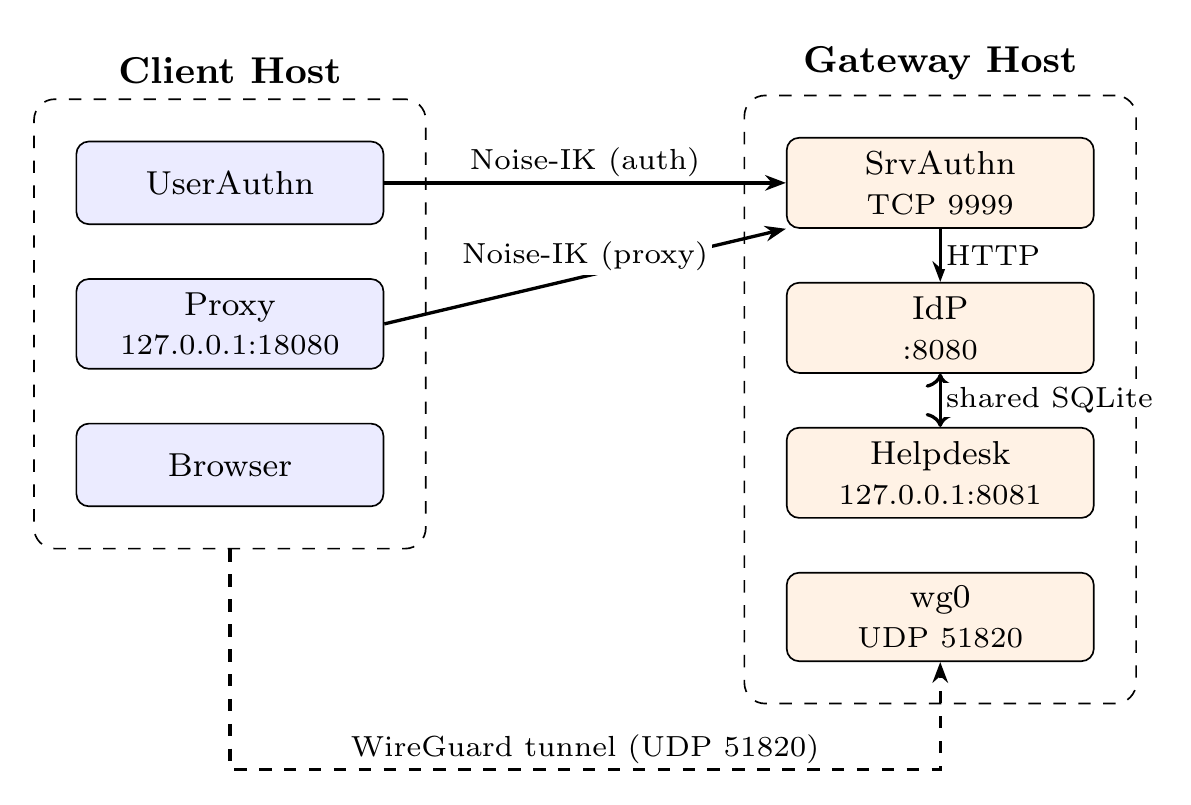
\includegraphics[width=0.95\textwidth]{architecture}
    \fbox{\parbox{0.9\textwidth}{\centering\vspace{3cm}
        \textit{TODO: Inserir diagrama de arquitetura}
    \vspace{3cm}}}
    \caption{Diagrama de componentes do sistema.}
    \label{fig:architecture}
\end{figure}

% ══════════════════════════════════════════════════════════════════════════════
\section{Modelo de confiança}
\label{sec:trust}

A única raiz de confiança é a chave pública WireGuard do gateway --- um
valor Curve25519 de 32~bytes. Esta chave desempenha dois papéis:

\begin{enumerate}
    \item \textbf{Chave estática do responder Noise-IK} para o túnel de
    autenticação. O \emph{handshake} falha se o servidor não provar posse
    da chave privada correspondente.
    \item \textbf{Chave estática WireGuard} para o plano de dados, usada
    pelo kernel após o túnel ser provisionado.
\end{enumerate}

Não existe TLS em nenhum ponto do sistema. O browser acede ao IdP através
de um proxy HTTP local que reutiliza o mesmo túnel Noise-IK (secção
\ref{sec:proxy}), eliminando a necessidade de certificados adicionais.

% ══════════════════════════════════════════════════════════════════════════════
\section{Fluxo de autenticação ponto-a-ponto}
\label{sec:flow}

O fluxo completo, desde o arranque do cliente até ao túnel VPN ativo:

\begin{enumerate}
    \item O UserAuthn gera uma PSK localmente (\texttt{wg genpsk}).
    \item Abre um túnel Noise-IK (TCP~9999) para o SrvAuthn, autenticado
          pela chave pública WireGuard do servidor.
    \item O SrvAuthn inicia o fluxo OAuth Device Grant junto do IdP
          (\texttt{POST /oauth/device/code}).
    \item O UserAuthn recebe o \texttt{user\_code} e o
          \texttt{verification\_uri} e abre o browser automaticamente.
    \item O browser liga-se ao proxy HTTP local
          (\texttt{127.0.0.1:18080}), que encaminha o tráfego pelo túnel
          Noise-IK até ao IdP.
    \item O utilizador submete o código e inicia o fluxo MFA:
    \begin{itemize}
        \item O IdP calcula a pontuação de risco (RBA).
        \item O \emph{PAM bridge} invoca \texttt{pam\_authenticate("iaa-vpn", ...)}.
        \item O módulo \texttt{pam\_vpnmfa.so} determina o tier (L1/L2/L3)
              e emite os fatores necessários via conversação PAM.
        \item Para cada fator, o IdP apresenta o formulário correspondente
              ao browser e submete o resultado (\texttt{OK}/\texttt{FAIL}/\texttt{UNAVAILABLE}).
    \end{itemize}
    \item Após sucesso MFA, o IdP emite um \emph{access token}.
    \item O SrvAuthn obtém o token via polling, gera o par de chaves WG
          do cliente, aloca um IP do \emph{subnet} \texttt{10.10.10.0/24}
          e executa \texttt{wg set wg0 peer ...}.
    \item Os parâmetros WG são enviados ao UserAuthn pelo túnel Noise.
    \item O UserAuthn escreve \texttt{wg0.conf} e executa
          \texttt{wg-quick up wg0} --- o túnel VPN fica ativo.
\end{enumerate}

% TODO: Insert flow diagram or screenshot of terminal + browser during auth
\begin{figure}[H]
    \centering
    % \includegraphics[width=0.95\textwidth]{auth_flow}
    \fbox{\parbox{0.9\textwidth}{\centering\vspace{3cm}
        \textit{TODO: Inserir capturas do fluxo de autenticação}
    \vspace{3cm}}}
    \caption{Fluxo de autenticação completo.}
    \label{fig:auth-flow}
\end{figure}

% ══════════════════════════════════════════════════════════════════════════════
\section{Túnel Noise-IK}
\label{sec:noise}

A comunicação entre o UserAuthn e o SrvAuthn utiliza o protocolo
\textbf{Noise-IK} (Noise Protocol Framework, revisão~34), implementado
de raiz em \texttt{common/noise.py} sem recurso a bibliotecas Noise
de terceiros. Os primitivos criptográficos são fornecidos pela biblioteca
\texttt{cryptography} (hazmat):

\begin{itemize}
    \item \textbf{Curve25519} --- troca de chaves Diffie-Hellman.
    \item \textbf{ChaCha20-Poly1305} --- cifra AEAD para o transporte.
    \item \textbf{BLAKE2s} --- função de hash para o estado do handshake.
\end{itemize}

O padrão IK garante que o iniciador conhece a chave estática do responder
\emph{a priori} --- no nosso caso, a chave pública WireGuard. As duas
mensagens do \emph{handshake}:

\begin{enumerate}
    \item \texttt{-> e, es, s, ss} --- o iniciador envia chave efémera,
    DH com estática do responder, a sua estática cifrada e DH mútuo.
    \item \texttt{<- e, ee, se} --- o responder responde com chave efémera
    e os DH restantes.
\end{enumerate}

Após o \emph{handshake}, cada direção tem o seu próprio
\texttt{CipherState} (ChaCha20-Poly1305 com nonce incremental). Todas
as mensagens subsequentes são frames com comprimento prefixado
(\texttt{common/framing.py}: 4~bytes big-endian + payload, limite de
64~KiB).

% ══════════════════════════════════════════════════════════════════════════════
\section{Proxy HTTP local}
\label{sec:proxy}

Para que o browser não necessite de contactar diretamente o gateway (o
que exigiria TLS e certificados), o UserAuthn implementa um proxy HTTP
local:

\begin{itemize}
    \item O \texttt{client/proxy.py} escuta em \texttt{127.0.0.1:18080}.
    \item Para cada ligação do browser, abre um \emph{novo} túnel Noise-IK
    ao SrvAuthn com \texttt{\{"service":"proxy"\}} como primeiro frame.
    \item O \texttt{server/proxy.py} abre uma ligação TCP ao IdP em
    \texttt{localhost:8080} e faz \emph{relay} bidirecional.
\end{itemize}

O \texttt{ORIGIN} do IdP é \texttt{http://localhost:18080}, pelo que
o \texttt{verification\_uri\_complete} gerado aponta para o proxy. O
browser abre esse URL; o tráfego flui sobre Noise-IK; o utilizador
nunca vê o endereço real do gateway.

% ══════════════════════════════════════════════════════════════════════════════
\section{Fatores de autenticação (MFA)}
\label{sec:mfa}

Três fatores são implementados, por ordem crescente de robustez:

\subsection{Palavra-passe --- desafio-resposta}
\label{sec:password}

A palavra-passe nunca abandona o browser em texto claro. O protocolo:

\begin{enumerate}
    \item \textbf{Registo (helpdesk):}
    \begin{itemize}
        \item \texttt{salt = os.urandom(16)}
        \item \texttt{verifier = scrypt(password, salt, N=$2^{14}$, r=8, p=1)} $\rightarrow$ 32~bytes
        \item Armazena \texttt{(salt, verifier)}.
    \end{itemize}

    \item \textbf{Login (IdP):}
    \begin{itemize}
        \item O servidor envia \texttt{(salt, nonce, parâmetros scrypt)}.
        \item O browser calcula \texttt{verifier' = scrypt(password, salt)}.
        \item O browser calcula \texttt{proof = HMAC-SHA256(verifier', nonce)}.
        \item O servidor verifica: \texttt{expected = HMAC-SHA256(verifier, nonce)},
              comparação em tempo constante.
        \item O \texttt{nonce} é marcado como consumido atomicamente
              (\texttt{BEGIN IMMEDIATE}) --- replay impossível.
    \end{itemize}
\end{enumerate}

O scrypt no browser é implementado em JavaScript puro
(\texttt{idp/static/js/scrypt.js}), seguindo o RFC~7914.

\subsection{TOTP}
\label{sec:totp}

RFC~6238: código de 6 dígitos, janela de 30~segundos, tolerância de $\pm$1
\emph{step}. O segredo partilhado é armazenado \textbf{cifrado em repouso}
com AES-256-GCM (secção~\ref{sec:hardening}).

\subsection{FIDO2 / WebAuthn}
\label{sec:fido2}

Utiliza a biblioteca \texttt{webauthn~$\geq$~2.0}. Tanto o registo (helpdesk)
como a autenticação (IdP) exigem
\texttt{UserVerificationRequirement.REQUIRED}, o que obriga o autenticador
a realizar verificação local (PIN ou biometria). Uma chave de segurança
roubada, sem PIN, não satisfaz este fator.

% TODO: Insert screenshots of each MFA factor form
\begin{figure}[H]
    \centering
    % \includegraphics[width=0.48\textwidth]{mfa_password}
    % \includegraphics[width=0.48\textwidth]{mfa_totp}
    \fbox{\parbox{0.45\textwidth}{\centering\vspace{2.5cm}
        \textit{TODO: Password form}
    \vspace{2.5cm}}}
    \hfill
    \fbox{\parbox{0.45\textwidth}{\centering\vspace{2.5cm}
        \textit{TODO: TOTP form}
    \vspace{2.5cm}}}
    \caption{Formulários MFA: palavra-passe (esq.) e TOTP (dir.).}
    \label{fig:mfa-forms}
\end{figure}

% ══════════════════════════════════════════════════════════════════════════════
\section{Orquestração PAM}
\label{sec:pam}

A especificação exige que a orquestração MFA e RBA seja feita com PAM.
A implementação segue esta arquitetura:

\subsection{Módulo PAM customizado}

O ficheiro \texttt{idp/pam\_iaa/src/pam\_vpnmfa.c} é compilado em
\texttt{pam\_vpnmfa.so} e instalado como módulo PAM. O perfil
\texttt{/etc/pam.d/iaa-vpn} contém:

\begin{lstlisting}[language=bash,caption={Perfil PAM \texttt{iaa-vpn}}]
# PAM service for the IAA VPN MFA orchestrator
auth    required    pam_vpnmfa.so
\end{lstlisting}

\subsection{Funcionamento}

\begin{enumerate}
    \item O IdP calcula a pontuação de risco e define
    \texttt{IAA\_RISK\_SCORE} como variável de ambiente PAM.
    \item O \emph{PAM bridge} (\texttt{idp/pam\_bridge.py}) invoca
    \texttt{pam\_authenticate} numa thread dedicada.
    \item O módulo C lê \texttt{IAA\_RISK\_SCORE}, determina o tier e
    emite mensagens \texttt{FACTOR:<nome>} pela função de conversação.
    \item O Python bridge espera em \texttt{threading.Event}; o Flask
    renderiza o formulário correspondente e submete o resultado.
\end{enumerate}

\subsection{Contrato de conversação}

\begin{table}[H]
\centering
\caption{Protocolo de conversação PAM.}
\label{tab:pam-conv}
\begin{tabular}{lll}
\toprule
\textbf{Estilo} & \textbf{Mensagem} & \textbf{Resposta esperada} \\
\midrule
\texttt{PAM\_PROMPT\_ECHO\_OFF} & \texttt{FACTOR:password} & \texttt{OK} / \texttt{FAIL} / \texttt{UNAVAILABLE} \\
\texttt{PAM\_PROMPT\_ECHO\_OFF} & \texttt{FACTOR:totp}     & \texttt{OK} / \texttt{FAIL} / \texttt{UNAVAILABLE} \\
\texttt{PAM\_PROMPT\_ECHO\_OFF} & \texttt{FACTOR:fido2}    & \texttt{OK} / \texttt{FAIL} / \texttt{UNAVAILABLE} \\
\texttt{PAM\_TEXT\_INFO}       & \texttt{INFO:tier=L2 ...} & (qualquer string) \\
\bottomrule
\end{tabular}
\end{table}

\subsection{Mapeamento de tiers}

\begin{table}[H]
\centering
\caption{Mapeamento de pontuação de risco para tiers e fatores.}
\label{tab:tiers}
\begin{tabular}{lcl}
\toprule
\textbf{Tier} & \textbf{Pontuação} & \textbf{Fatores exigidos} \\
\midrule
L1 & $< 30$    & Palavra-passe \\
L2 & $< 60$    & Palavra-passe + TOTP \\
L3 & $\geq 60$ & Palavra-passe + TOTP + FIDO2 \\
\bottomrule
\end{tabular}
\end{table}

% ══════════════════════════════════════════════════════════════════════════════
\section{Autenticação baseada em risco (RBA)}
\label{sec:rba}

O motor de risco (\texttt{idp/rba.py}) agrega quatro sinais, todos
obtidos a partir de dados locais na base de dados --- sem chamadas a
APIs externas:

\begin{table}[H]
\centering
\caption{Sinais do motor de risco.}
\label{tab:rba-signals}
\begin{tabular}{lcc}
\toprule
\textbf{Sinal} & \textbf{Penalização} & \textbf{Origem} \\
\midrule
Primeiro login do utilizador     & +0.30        & \texttt{rba\_ip\_history} vazia \\
IP novo (utilizador existente)   & +0.20        & IP ausente de \texttt{rba\_ip\_history} \\
Falhas recentes (últimos 30 min) & +0.10 cada (máx. +0.40) & \texttt{rba\_events} \\
Hora invulgar (00:00--06:00 UTC) & +0.20        & \texttt{datetime.now().hour} \\
\bottomrule
\end{tabular}
\end{table}

A pontuação final é limitada ao intervalo $[0, 1]$ e escalada para $[0, 100]$
para o módulo PAM. Se o tier exigido requerer um fator para o qual o
utilizador não está inscrito, o sistema retorna erro 403 sem degradar
silenciosamente para um tier inferior.

% ══════════════════════════════════════════════════════════════════════════════
\section{Camada de dados}
\label{sec:data}

Base de dados SQLite única em \texttt{/data/vpnauth.db} (modo WAL, foreign
keys ativas), partilhada entre o IdP e o Helpdesk via \emph{bind mount}.

Três operações utilizam \texttt{BEGIN IMMEDIATE} para evitar condições de
corrida:
\begin{itemize}
    \item \textbf{lease\_next\_ip} --- alocação atómica de IP.
    \item \textbf{consume\_password\_nonce} --- queima atómica do nonce de
    desafio-resposta.
    \item \textbf{mark\_token\_used} --- marcação atómica de token OAuth
    como usado.
\end{itemize}

% ══════════════════════════════════════════════════════════════════════════════
\section{Robustecimento de segurança}
\label{sec:hardening}

Para além dos requisitos da especificação, foram implementadas as seguintes
medidas de robustecimento:

\begin{description}[style=nextline]
    \item[Tokens OAuth hasheados em repouso]
    Armazenados como \texttt{SHA-256(token)}, TTL de 60~s, uso único
    (\texttt{used\_at} atualizado atomicamente).

    \item[Bloqueio de conta]
    5 falhas em 5~minutos bloqueiam a conta durante 15~minutos. O
    contador reseta após login bem-sucedido.

    \item[Segredos TOTP cifrados em repouso]
    AES-256-GCM com chave mestra (\texttt{IAA\_MASTER\_KEY}) validada
    no arranque.

    \item[Arranque \emph{fail-closed}]
    Todos os processos recusam arrancar com segredos em falta ou
    \emph{placeholder}.

    \item[Alocação de IP livre de corridas]
    \texttt{BEGIN IMMEDIATE} no SQLite garante que dois provisionamentos
    concorrentes não obtêm o mesmo IP.

    \item[Validação de formato de chaves WG]
    A PSK do cliente é decodificada de base64 e verificada como exatamente
    32~bytes antes de ser passada ao \texttt{wg set}.

    \item[Helpdesk apenas em loopback]
    O bind a \texttt{127.0.0.1} com \texttt{network\_mode: host} garante
    que o helpdesk é inacessível externamente.

    \item[Expiração de leases]
    Thread de \emph{sweeper} que remove peers expirados da interface
    \texttt{wg0}.
\end{description}

% ══════════════════════════════════════════════════════════════════════════════
\section{Testes e validação}
\label{sec:tests}

\subsection{Ambiente de teste}

Os testes foram realizados com Docker Compose em máquina Linux (Ubuntu 24.04).
O contentor \texttt{vpn-client} simula o host do utilizador com namespace de
rede próprio, permitindo testar o túnel WireGuard completo numa única máquina.

\subsection{Registo de utilizador (Helpdesk)}

% TODO: Insert helpdesk screenshots
\begin{figure}[H]
    \centering
    % \includegraphics[width=0.8\textwidth]{helpdesk_user}
    \fbox{\parbox{0.8\textwidth}{\centering\vspace{3cm}
        \textit{TODO: Captura do helpdesk com utilizador registado
        (password SET, TOTP CONFIRMED, FIDO2 1 KEY)}
    \vspace{3cm}}}
    \caption{Interface do Helpdesk com utilizador totalmente inscrito.}
    \label{fig:helpdesk}
\end{figure}

\subsection{Fluxo de autenticação completo}

% TODO: Insert auth flow screenshots (terminal + browser)
\begin{figure}[H]
    \centering
    % \includegraphics[width=0.8\textwidth]{terminal_auth}
    \fbox{\parbox{0.8\textwidth}{\centering\vspace{3cm}
        \textit{TODO: Captura do terminal com UserAuthn + user code}
    \vspace{3cm}}}
    \caption{Terminal do UserAuthn a apresentar o código do dispositivo.}
    \label{fig:terminal-auth}
\end{figure}

\begin{figure}[H]
    \centering
    % \includegraphics[width=0.8\textwidth]{browser_mfa}
    \fbox{\parbox{0.8\textwidth}{\centering\vspace{3cm}
        \textit{TODO: Captura do browser durante o fluxo MFA}
    \vspace{3cm}}}
    \caption{Browser a completar a autenticação multi-fator.}
    \label{fig:browser-mfa}
\end{figure}

\subsection{Túnel WireGuard ativo}

% TODO: Insert WG tunnel screenshots
\begin{figure}[H]
    \centering
    % \includegraphics[width=0.8\textwidth]{wg_show}
    \fbox{\parbox{0.8\textwidth}{\centering\vspace{2.5cm}
        \textit{TODO: Captura de \texttt{wg show wg0} no cliente e servidor}
    \vspace{2.5cm}}}
    \caption{Estado da interface WireGuard após autenticação.}
    \label{fig:wg-show}
\end{figure}

\begin{figure}[H]
    \centering
    % \includegraphics[width=0.8\textwidth]{ping_tunnel}
    \fbox{\parbox{0.8\textwidth}{\centering\vspace{2cm}
        \textit{TODO: Captura de \texttt{ping 10.10.10.1} bem-sucedido}
    \vspace{2cm}}}
    \caption{Ping através do túnel VPN confirmando conectividade.}
    \label{fig:ping}
\end{figure}

\subsection{Tiers de risco diferentes}

% TODO: Insert RBA tier comparison screenshots
\begin{figure}[H]
    \centering
    % \includegraphics[width=0.48\textwidth]{tier_l1}
    % \includegraphics[width=0.48\textwidth]{tier_l3}
    \fbox{\parbox{0.45\textwidth}{\centering\vspace{2.5cm}
        \textit{TODO: Login L1 (só password)}
    \vspace{2.5cm}}}
    \hfill
    \fbox{\parbox{0.45\textwidth}{\centering\vspace{2.5cm}
        \textit{TODO: Login L3 (3 fatores)}
    \vspace{2.5cm}}}
    \caption{Comparação de tiers: L1 (esq.) vs L3 (dir.).}
    \label{fig:tiers}
\end{figure}

\subsection{Bloqueio de conta}

% TODO: Insert lockout screenshot
\begin{figure}[H]
    \centering
    % 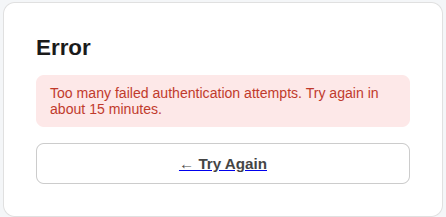
\includegraphics[width=0.6\textwidth]{lockout}
    \fbox{\parbox{0.6\textwidth}{\centering\vspace{2cm}
        \textit{TODO: Captura de conta bloqueada após 5 falhas}
    \vspace{2cm}}}
    \caption{Mensagem de bloqueio de conta.}
    \label{fig:lockout}
\end{figure}

\subsection{Dados cifrados em repouso}

% TODO: Insert DB query screenshots showing hashed/encrypted data
\begin{figure}[H]
    \centering
    % \includegraphics[width=0.8\textwidth]{encrypted_data}
    \fbox{\parbox{0.8\textwidth}{\centering\vspace{2cm}
        \textit{TODO: Queries à BD mostrando tokens hasheados, TOTP cifrado, verifier scrypt}
    \vspace{2cm}}}
    \caption{Dados sensíveis armazenados cifrados/hasheados na base de dados.}
    \label{fig:encrypted-data}
\end{figure}

% ══════════════════════════════════════════════════════════════════════════════
\section{Funcionalidades não implementadas}
\label{sec:not-impl}

\begin{itemize}
    \item \textbf{Indicador RBA ``Autonomous Service'' (AS/ASN).}
    A especificação lista \emph{``same/different Autonomous Service''}
    como um dos sinais de exemplo para RBA. Não foi implementado porque
    requereria incluir uma base de dados GeoIP/ASN ($\sim$50~MB) ou
    realizar chamadas a APIs externas em cada login --- o que constitui
    uma fuga de privacidade e uma dependência externa num sistema cujo
    modelo de confiança é deliberadamente fechado. A linguagem da
    especificação é ilustrativa (\emph{``consider using ... etc.''}),
    e os restantes três indicadores nomeados estão implementados.
\end{itemize}

% ══════════════════════════════════════════════════════════════════════════════
\section{Conclusão}
\label{sec:conclusion}

O sistema implementado cumpre todos os requisitos obrigatórios da
especificação do projeto: autenticação de utilizadores WireGuard com
três fatores MFA (palavra-passe por desafio-resposta, TOTP e FIDO2),
orquestração via módulo PAM customizado, autenticação baseada em risco,
e provisionamento dinâmico de parâmetros WireGuard sobre um fluxo
OAuth~2.0 Device Authorization Grant.

A raiz de confiança é a chave pública WireGuard do gateway, utilizada
simultaneamente como chave estática Noise-IK e como chave do plano de
dados, eliminando a necessidade de TLS, certificados ou infraestrutura
PKI.

Adicionalmente, foram implementadas medidas de robustecimento além do
especificado: tokens hasheados e de uso único, bloqueio de conta,
cifra de segredos TOTP em repouso, arranque \emph{fail-closed} e
expiração automática de leases.

% ══════════════════════════════════════════════════════════════════════════════
\section{Contribuições}
\label{sec:contributions}

% TODO: Fill in before submission
\begin{table}[H]
\centering
\caption{Contribuições dos autores.}
\label{tab:contributions}
\begin{tabular}{clc}
\toprule
\textbf{Número} & \textbf{Nome} & \textbf{Contribuição} \\
\midrule
XXXXX & Nome Autor 1 & XX\% \\
XXXXX & Nome Autor 2 & XX\% \\
XXXXX & Nome Autor 3 & XX\% \\
\bottomrule
\end{tabular}
\end{table}

% ══════════════════════════════════════════════════════════════════════════════
\section{Código de terceiros}
\label{sec:third-party}

\textbf{Trabalho original:} implementação Noise-IK
(\texttt{common/noise.py}), scrypt no browser
(\texttt{idp/static/js/scrypt.js}), módulo PAM
(\texttt{pam\_vpnmfa.c}), wrapper ctypes libpam
(\texttt{common/libpam.py}), e todo o restante código em
\texttt{client/}, \texttt{server/}, \texttt{idp/}, \texttt{common/}
e \texttt{scripts/}.

\begin{table}[H]
\centering
\caption{Bibliotecas externas utilizadas.}
\label{tab:third-party}
\begin{tabularx}{\textwidth}{lX}
\toprule
\textbf{Biblioteca} & \textbf{Utilização} \\
\midrule
\texttt{flask}          & Servidor HTTP para o IdP e helpdesk \\
\texttt{pyotp}          & Geração e verificação TOTP (RFC~6238) \\
\texttt{webauthn}       & Verificação WebAuthn / FIDO2 \\
\texttt{qrcode, pillow} & Códigos QR para registo TOTP \\
\texttt{cryptography}   & X25519, ChaCha20-Poly1305, AES-256-GCM, BLAKE2s \\
\bottomrule
\end{tabularx}
\end{table}

Ferramentas de sistema invocadas por subprocesso: \texttt{wg},
\texttt{wg-quick}, \texttt{wg genkey}, \texttt{wg pubkey},
\texttt{wg genpsk}.

\end{document}
